\iffalse
\chapter{2015}
\author{AI24BTECH11030}
\section{ph}
\fi

\item
A particle of mass \(0.01 \, \text{kg}\) falls freely in the earth's gravitational field with an initial velocity \( v(0) = 10 \, \text{ms}^{-1} \). If the air exerts a frictional force of the form, \( f = -kv \), then for \( k = 0.05 \, \text{Nm}^{-1} \cdot \text{s} \), the velocity (in \(\text{ms}^{-1}\)) at time \( t = 0.2 \, \text{s} \) is \ldots\ldots (up to two decimal places). (use \( g = 10 \, \text{ms}^{-2} \) and \( e = 2.72 \)) \hfill (GATE PH 2015)

\item
In the nuclear shell model, the potential is modeled as
\(
V(r) = \frac{1}{2} m \omega^2 r^2 - \lambda \, \vec{L} \cdot \vec{S}, \lambda > 0.
\)
The correct spin-parity and isospin assignments for the ground state of \( ^{13}\text{C} \) is \hfill (GATE PH 2015)

\begin{multicols}{4}
    \begin{enumerate}
        \item \( \frac{1}{2}^- ; -\frac{1}{2} \)
        \item \( \frac{1}{2}^+ ; -\frac{1}{2} \)
        \item \( \frac{3}{2}^+ ; -\frac{1}{2} \)
        \item \( \frac{3}{2}^- ; -\frac{1}{2} \)
    \end{enumerate}
\end{multicols}

\item
A particle is confined in a box of length \( L \) as shown below.

\begin{center}
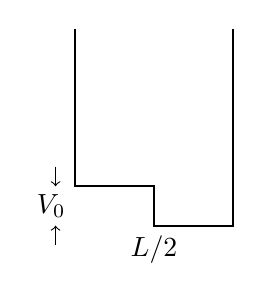
\begin{tikzpicture}
    % Draw the box
    \draw[thick] (0,0) -- (0, -2) -- (1, -2) -- (1, -2.5) -- (2,-2.5) -- (2,0);

    % % Mark the L/2 and L points
    \node[below] at (1,-2.5) {\(L/2\)};
    \draw[->] (-0.25,-1.75) -- (-0.25,-2);
    \node[left] at (0,-2.25) {\(V_0\)};
    \draw[->] (-0.25,-2.75) -- (-0.25,-2.5);
\end{tikzpicture}
\end{center}

If the potential \( V_0 \) is treated as a perturbation, including the first order correction, the ground state energy is \hfill (GATE PH 2015)

\begin{multicols}{4}
    \begin{enumerate}
        \item \( E = \frac{\hbar^2 \pi^2}{2mL^2} + V_0 \)
        \item \( E = \frac{\hbar^2 \pi^2}{2mL^2} - \frac{V_0}{2} \)
        \item \( E = \frac{\hbar^2 \pi^2}{2mL^2} + \frac{V_0}{4} \)
        \item \( E = \frac{\hbar^2 \pi^2}{2mL^2} + \frac{V_0}{2} \)
    \end{enumerate}
\end{multicols}

\item

Suppose a linear harmonic oscillator of frequency \( \omega \) and mass \( m \) is in the state
\[
\vert{\psi}\rangle = \frac{1}{\sqrt{2}} \brak{ \vert{\psi_0}\rangle + e^{\frac{\pi}{2}} \vert{\psi_1}\rangle } \text{ at } t = 0
\]
where \( \vert{\psi_0}\rangle \) and \( \vert{\psi_1}\rangle \) are the ground and the first excited states, respectively. The value of \( \langle{\psi | x | \psi}\rangle \) in the units of \( \sqrt{\frac{\hbar}{m \omega}} \) at \( t = 0 \) is \ldots\ldots. \hfill (GATE PH 2015)

\item A particle with rest mass \( M \) is at rest and decays into two particles of equal rest masses \( \frac{3}{10} M \) which move along the \( z \) axis. Their velocities are given by \hfill (GATE PH 2015)

\begin{multicols}{2}
    \begin{enumerate}
        \item \( \vec{v}_1 = \vec{v}_2 = (0.8c) \hat{z} \)
        \item \( \vec{v}_1 = -\vec{v}_2 = (0.8c) \hat{z} \)
        \item \( \vec{v}_1 = -\vec{v}_2 = (0.6c) \hat{z} \)
        \item \( \vec{v}_1 = (0.6c) \hat{z}; \quad \vec{v}_2 = (-0.8c) \hat{z} \)
    \end{enumerate}
\end{multicols}

\item In the given circuit, if the open loop gain \( A = 10^5 \), the feedback configuration and the closed loop gain \( A_f \) are

\begin{center}
    \resizebox{0.25\textwidth}{!}{
    \begin{circuitikz}
        % \node[op amp, noinv input up] (opamp) at (0,0) {};
        % \draw (opamp.+) -- ++(-0.5,0) node {$v_i$};

        \draw (0,0) node[op amp, yscale=-1] (opamp) {}
        (opamp.+) node[left] {$V_i$}
        (opamp.out) -- ++(0.5,0) node[right] {$V_o$};

        % Draw resistors and connections
        \draw (opamp.-) -- ++(-0.5,0) -- ++(0,-1) to[R=9~k$\Omega$] ++(+2.9,0);

        \draw (opamp.-) -- ++(-0.5,0) -- ++(0,-1) to[R=1~k$\Omega$] ++(0,-2) node[ground]{};

        \draw (opamp.out) -- ++(0,-1.6) to[R=$R_L$] ++(0,-2) node[ground]{};
    \end{circuitikz}}
\end{center}
\hfill (GATE PH 2015)

\begin{multicols}{2}
    \begin{enumerate}
        \item series-shunt, \( A_f = 9 \)
        \item series-series, \( A_f = 10 \)
        \item series-shunt, \( A_f = 10 \)
        \item shunt-shunt, \( A_f = 10 \)
    \end{enumerate}
\end{multicols}

\item A function $y(z)$ satisfies the ordinary differential equation
$$ y'' + \frac{1}{z} y' - \frac{m^2}{z^2} y = 0, $$
where $m = 0,1,2,3, \dots$. Consider the four statements $P$, $Q$, $R$, $S$ as given below.

\begin{enumerate}
    \item[P:] $z^m$ and $z^{-m}$ are linearly independent solutions for all values of $m$
    \item[Q:] $z^m$ and $z^{-m}$ are linearly independent solutions for all values of $m > 0$
    \item[R:] $\ln z$ and 1 are linearly independent solutions for $m = 0$
    \item[S:] $z^m$ and $\ln z$ are linearly independent solutions for all values of $m$
\end{enumerate}

The correct option for the combination of valid statements is \hfill (GATE PH 2015)
\begin{multicols}{4}
    \begin{enumerate}
        \item P, R and S only
        \item P and R only
        \item Q and R only
        \item R and S only
    \end{enumerate}
\end{multicols}

\item The entropy of a gas containing $N$ particles enclosed in a volume $V$ is given by $ S = N k_B \ln \brak{ \frac{a V E^{\frac{3}{2}}}{N^{\frac{5}{2}}} }, $ where $E$ is the total energy, $a$ is a constant, and $k_B$ is the Boltzmann constant. The chemical potential $\mu$ of the system at a temperature $T$ is given by \hfill (GATE PH 2015)

\begin{multicols}{2}
    \begin{enumerate}
        \item $\mu = -k_B T \sbrak{ \ln \brak{ \frac{a V E^{\frac{3}{2}}}{N^{\frac{5}{2}}} } - \frac{5}{2} }$
        \item $\mu = -k_B T \sbrak{ \ln \brak{ \frac{a V E^{\frac{3}{2}}}{N^{\frac{5}{2}}} } - \frac{3}{2} }$
    
        \item $\mu = -k_B T \sbrak{ \ln \brak{ \frac{a V E^{\frac{3}{2}}}{N^{\frac{3}{2}}} } - \frac{5}{2} }$
        \item $\mu = -k_B T \sbrak{ \ln \brak{ \frac{a V E^{\frac{3}{2}}}{N^{\frac{3}{2}}} } - \frac{3}{2} }$
    \end{enumerate}
\end{multicols}

\item  Let the Hamiltonian for two spin-$\frac{1}{2}$ particles of equal masses $m$, momenta $\bm{p}_1$ and $\bm{p}_2$, and positions $\bm{r}_1$ and $\bm{r}_2$ be 
$$ H = \frac{1}{2m} p_1^2 + \frac{1}{2m} p_2^2 + \frac{1}{2} m \omega^2 (r_1^2 + r_2^2) + k \bm{\sigma}_1 \cdot \bm{\sigma}_2, $$
where $\bm{\sigma}_1$ and $\bm{\sigma}_2$ denote the corresponding Pauli matrices, $\hbar \omega = 0.1 \, \text{eV}$ and $k = 0.2 \, \text{eV}$. If the ground state has net spin zero, then the energy (in eV) is \ldots\ldots. \hfill (GATE PH 2015)

\item The average energy $U$ of a one dimensional quantum oscillator of frequency $\omega$ and in contact with a heat bath at temperature $T$ is given by \hfill (GATE PH 2015)

\begin{multicols}{2}
    \begin{enumerate}
        \item $U = \frac{1}{2} \hbar \omega \coth \brak{ \frac{1}{2} \beta \hbar \omega }$
        \item $U = \frac{1}{2} \hbar \omega \sinh \brak{ \frac{1}{2} \beta \hbar \omega }$
        \item $U = \frac{1}{2} \hbar \omega \tanh \brak{ \frac{1}{2} \beta \hbar \omega }$
        \item $U = \frac{1}{2} \hbar \omega \cosh \brak{ \frac{1}{2} \beta \hbar \omega }$
    \end{enumerate}
\end{multicols}

\item  A monochromatic plane wave (wavelength $= 600 \, \text{nm}$) $E_0 \exp[i(kz - \omega t)]$ is incident normally on a diffraction grating giving rise to a plane wave $E_1 \exp \sbrak{ i \brak{ \bm{k}_1 \cdot \bm{r} - \omega t } }$ in the first order of diffraction. Here $E_1 < E_0$ and $\bm{k}_1 = \lvert \bm{k}_1 \rvert \sbrak{ \frac{1}{2} \hat{x} + \frac{\sqrt{3}}{2} \hat{z} }$. The period (in $\mu \text{m}$) of the diffraction grating is \ldots\ldots (upto one decimal place) \hfill (GATE PH 2015)

\item The Heaviside function is defined as 
$ H(t) = \begin{cases} 
    +1 & \text{for } t > 0 \\
    -1 & \text{for } t < 0 
\end{cases}$
and its Fourier transform is given by $-\frac{2i}{\omega}$. The Fourier transform of $\frac{1}{2} \sbrak{ H(t + 1/2) - H(t - 1/2) }$ is \hfill (GATE PH 2015)

\begin{multicols}{4}
    \begin{enumerate}
        \item $\frac{\sin \brak{ \frac{\omega}{2} }}{\frac{\omega}{2}}$
        \item $\frac{\cos \brak{ \frac{\omega}{2} }}{\frac{\omega}{2}}$
        \item $\sin \brak{ \frac{\omega}{2} }$
        \item $0$
    \end{enumerate}
\end{multicols}

\item The atomic masses of ${}^{152}_{63}\text{Eu}$, ${}^{152}_{62}\text{Sm}$, ${}^{1}_{1}\text{H}$ and neutron are 151.921749, 151.919756, 1.007825 and 1.008665 in atomic mass units (amu), respectively. Using the above information, the $Q$-value of the reaction ${}^{152}_{63}\text{Eu} + n \rightarrow {}^{152}_{62}\text{Sm} + p$ is \ldots\ldots $\times 10^{-3}$ amu (up to three decimal places) \hfill (GATE PH 2015)
